\newpage
\section{Accessible}
\subsection*{}
 
Los datos se consideran accesibles por el usuario cuando este no necesita realizar un esfuerzo desmesurado para
poder obtenerlos, entenderlos y usarlos, es decir, aplicarlos a su situacion particular. Para lograr estos objetivos,
es necesario que el usuario pueda acceder a ellos de una manera que le resulte familiar y en un lenguage y nomenclatura
que pueda entender.\\ 

En este apartado veremos si es posible el acceso a los datos por un usuario medio y como optimizar la accesibilidad.

\subsection{Disponibilidad vs Accesibilidad.}
    
Como mencionamos en la introduccion de este capitulo, los datos pueden estar disponibles en la fuente original, pero no por
ello significa que estos sean accesibles.
Los retos a los que nos encontramos con los datos crudos, directos de la fuente de origen, son los siguientes:
    
    \begin{itemize}
        \item \textbf{Localizacion}. Los datos se encuentran disponibles en portales de datos abiertos organizados 
        y estructurados, normalmente se necesita una tarea de busqueda y seleccion
        a veces complicada. Aunque las empresas ponen cada vez mas de su parte en ofrecer una interfaz 
        agradable y funcional a los usuarios, esta tarea requiere de un trabajo de investigacion por parte del usuario,
        ya que posiblemente, debera buscar en distintos portales.
        \item \textbf{Extraccion}. Los datos suelen estan disponibles a traves de una interfaz de programacion 
        de aplicaciones (API) no facilmente interpretable por el usuario medio. Normalmente cuenta con 
        un documento que describe cada uno de los campos y valores que se presentan en el documento y como utilizar la API.
        \item \textbf{Interpretabilidad}. Usualmente los datos estan representados en un formato para ser procesado por 
        algun software, por lo que su lectura resulta complicada por el usuario medio, en el mejor de los casos, 
        estaran representados en una tabla y aun asi, sera muy dificil de extraer informacion.
        \item \textbf{Infraestructura}. Por ejemplo, el almacenamiento. Los datos publicados son los mas recientes, por lo que no hay manera de obtener 
        un historico de los datos si no son almacenados periodicamente. Una vez extraidos los datos, el usuario debera 
        contar con una infraestructura que le permita almacenar los datos.
        \item \textbf{Automatizacion}. Este proceso tiende a ser arduo, por lo que sera necesario automatizarlo, de otra 
        forma el esfuerzo requerido por el usuario para extraer la informacion no le compensara. 
        \item \textbf{Awarenes}. El usuario necesitara saber que tiene este recurso y puede utilizarlo.
         
    \end{itemize}
    
Por lo tanto, no podemos decir que estos datos sean accesibles de una forma util para el usuario medio.\\
\subsubsection{How to solve it.} 

Deberemos proporcionar la informacion requerida por el usuario de forma directa, facil de leer e interpretar. Ademas proporcionaremos
la infraestructura necesaria para que el usuario solo tenga que consultar los datos y automatizaremos los procesos que deban repetirse
periodicamente.
 
\subsubsection{How we solve it. Aire Guru.} 

Nuestra herramienta utiliza los datos de calidad del aire proporcionados por el ayuntamiento de Malaga en su portal de datos abiertos.\footnote{\url{https://datosabiertos.malaga.eu/}}\\
\begin{figure}[h]
    \centering
   \subfigure[Pagina principal]
    {\includegraphics[width=5.5cm  ]{OpenDataPortal}}
    \hfill
    \subfigure [Categoria medio ambiente]
       { 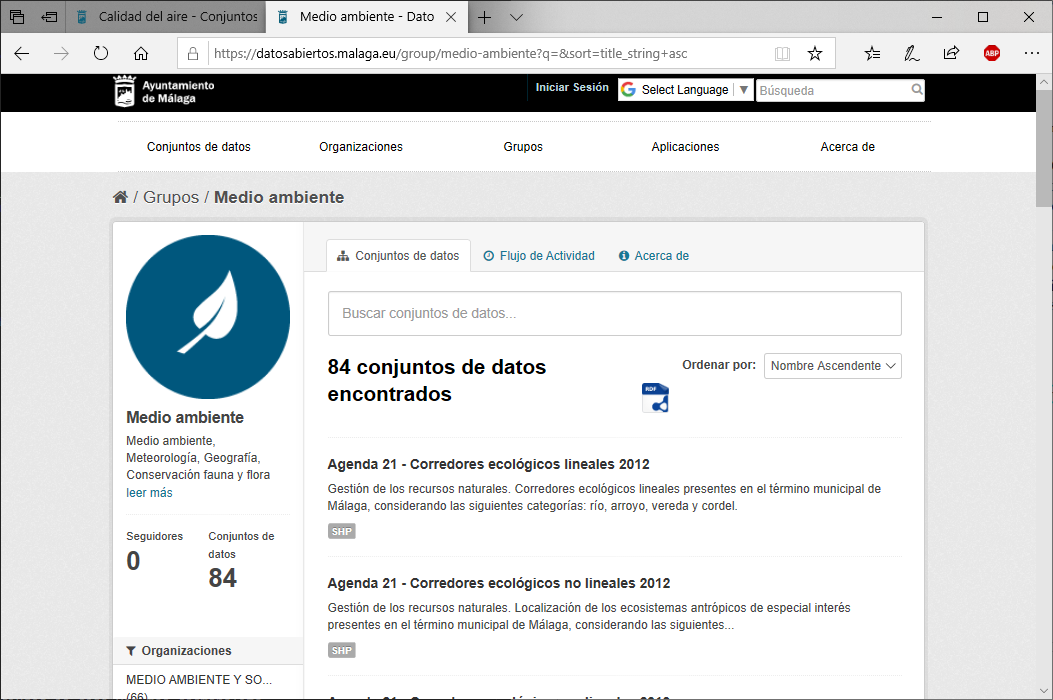
\includegraphics[width=5.5cm]{openDataPortalEnviromentCategory}}
    \vfill
     \subfigure[GeoJson Document]
     { \centering 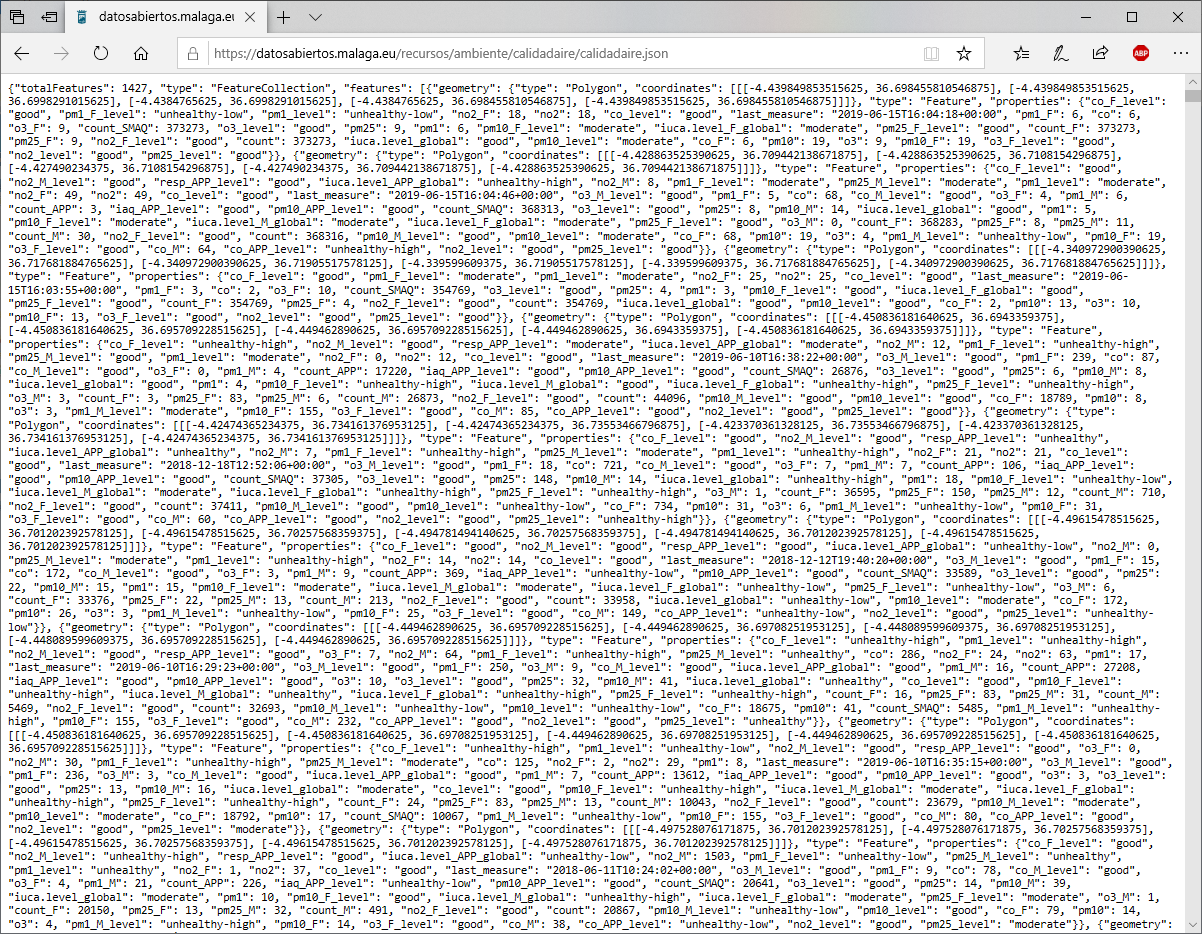
\includegraphics[width=4.75cm]{geoJsonAirQualityDataRaw}}
  
  \caption{Open Data Portal Malaga}
    \end{figure}

    Este portal de datos ofrece una oferta de categorias representados por iconos, por lo que es necesario saber en que categoria se clasifica el conjunto
de datos, una vez que se accede a la categoria, tenemos una barra buscadora que nos permite insertar las palabras claves para buscar el conjunto de datos
deseado.\\

En este caso puede pulsarse sobre el enlace y este abrira los datos en una nueva pestana, por lo que la utilizacion de un sistema informatico
para la descarga de los datos no es extrictamente necesario, pero podemos ver que ver que el formato no es legible, al menos desde el punto
de vista humano. 
Se actualiza cada hora, por lo que si queremos acceder a unos datos en concreto, deberemos repetir la operacion periodicamente.
Un valor importante de este conjunto de datos es saber la evolucion de la polucion por zonas, la extraccion de esta informacion no es posible
si no se realiza un almacenado de los datos.

Aire Guru automatiza el proceso de recoleccion de los datos mediante un trabajo CRON que ejecuta un script implementado en JavaScript periodicamente. Este lee 
los datos de la url, los procesa, limpia y almacena en una base de datos MongoDB.

\begin{figure}[ht]
    \centering
    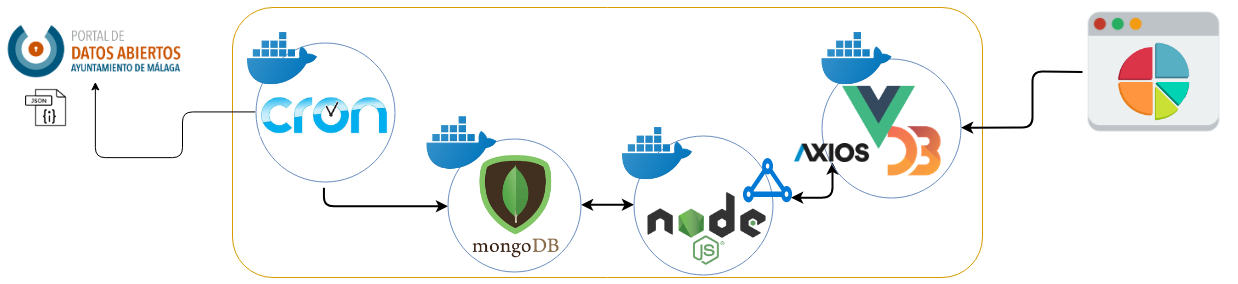
\includegraphics[width=12cm]{aireGuruArquitecture}
    \caption{Arquitecture Aire Guru}
\end{figure}

Mediante una interfaz web, muestra los datos al usuarios.

\begin{figure}[ht]
    \centering
    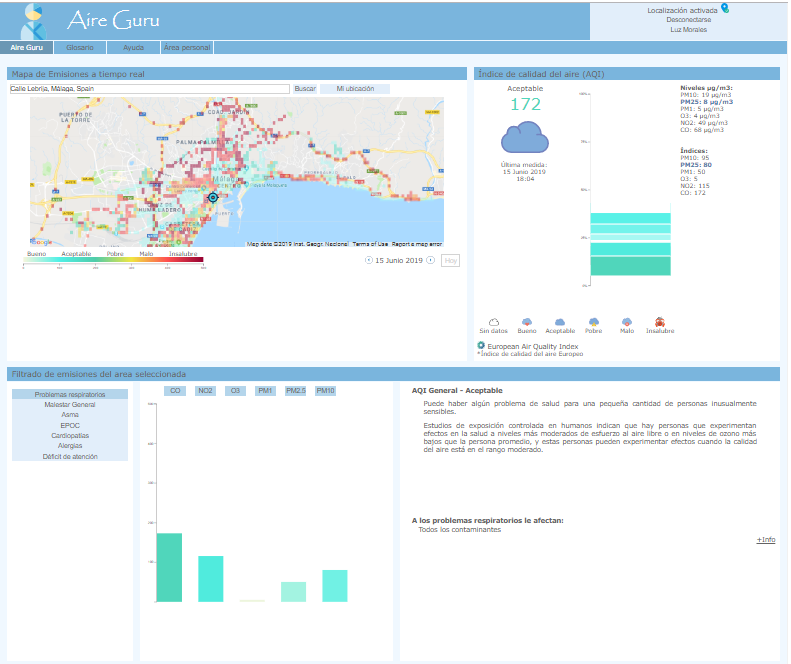
\includegraphics[width=9cm]{aireGuru}
    \caption{Aire Guru. Web Interface}
\end{figure}

Actualmente se trabaja en dar a conocer este producto. De momento esta disponible en el portal de datos abiertos en la pestana de aplicaciones.
.\footnote{\url{https://datosabiertos.malaga.eu/aplicaciones}}\\


\paragraph{Evaluation} \mbox{}

\begin{itemize}
    \done Localizacion. La localizacion de los datos es directa, ya que ofrece informacion desde el primer momento en que se accede a la web. En la pagina principal
presenta los niveles de polucion en todas las zonas sin necesidad de realizar ninguna seleccion.
\done Extraccion. No es necesario ningun software o conocimientos informaticos para acceder la informacion.
\done Interpretabildad. Contine un mapa donde los niveles de polucion se presentan por colores. Estos colores estan definidos por una leyenda justo
debajo del mapa. Cuenta con un glosario donde se explica los conceptos expuesto en la pagina web, el significado de cada seccion y como
navegar por la pagina web.
\done Infraestructura. Implementa toda la arquitectura necesaria tanto de almacenaje, procesado como visualizacion.
\done Automatiza los procesos de recoleccion de datos y los calculos necesarios para mostrar la informacion al usuario. Por ejemplo, una pregunta simple 
seria saber a que nivel de polucion estamos rodeados en las coordenadas en la que nos encontramos. Con la informacion en crudo obtenida desde el portal, 
nos es una tarea imposible, pero si ardua si no contamos con un sistema que procese los datos. Aire Guru resulve este problema.
\crossed Awarenes. Deberia trabajarse en la publicidad de la plataforma y darla a conocer.
\end{itemize}
\newpage

 



\subsection{Formato}
El punto clave para que el usuario entienda lo que queremos transmitirle es crear una comunicacion fluida entre la representacion
de los datos el usuario. Para ello  deberemos asegurarnos que hablamos el mismo idioma, con un vocabulario facil de entender y
con proximidad, es decir,dejar la terminologia a un lado y comunicar el objetivo de la manera mas simple posible.
Por ello la representacion de la informacion jugaran un papel fundamental para que la 
informacion sea absorbida por el usuario de una manera natural.


\subsubsection{How to solve it} 
Este modelo debera proporcionar la informacion al usario en un lenguaje o formato compresible. Si no es posible proporcionaremos las 
herramientas necesarias para que este pueda comprender el contexto de la informacion.
Deberemos estudiar que tipo de representacion es mas adecuada, no siempre una grafica es la representacion mas adecuada, deberemos hacer un 
estudio de tanto al publico al que va dirigido como como podemos acentuar la informacion que sea mas relevante en la manera 
correcta.
Si nos declinamos por realizar una representacion con graficas, deberemos estudiar los datos para saber que tipo de grafica. Por ejemplo, 
si hablamos de muestras y queremos saber la densidad, nos inclinaremos por un grafico de densidad y si por ejemplo buscamos la diferencia 
entre sexos, utilizaremos un grafico de tartas.

\subsubsection{How we solve it. Aire Guru} 
La herramienta Aire guru presenta la informacion en el idioma nativo de la ciudad y se utiliza un lenguaje sencillo y directo.
See utiliza el mismo estilo, colores e iconografia en todo el diseno para que el usuario se familierize rapidamente y pueda
prestar atencion al significado de los datos en vez de perderse en el diseno e intentar encontrar su significado.//

Unos de los objetivos es representa la contaminacion por zonas de la ciudad, por lo que se ha utilizado un mapa sobre el que se representa
 el AQI general calculado. Este es un formato mas legible para los usuarios ya que no tiene que trabajar para realizar una imagen visual
 de los distintos lugares de la ciudad. Este indice mustra un indicador con cinco niveles representados por una escala de colores desde el 
 turquesa hasta el rojo ("Bueno" "Aceptable""Pobre" "Malo" e "Insalubre"). La razon de esta eleccion es porqu eson los colores oficiales y 
 asi se evita crear confusion al usuario.
 \newpage
 \begin{figure}[ht]
    \centering
    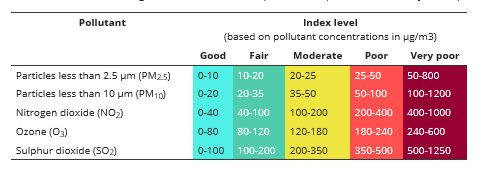
\includegraphics[width=12cm]{EAQI}
    \caption{EAQI Levels}
\end{figure}

Nuestra plataforma introduce ademas una iconografica para ayudar al usuario a tener una idea directa de la situacion, ya que son mas 
explicativos que los colores. En caso de peligro, queda bien representado con el color rojo, pero en el caso del azul o verde, en nuestra cultura, no
tenemos definido un estado para estos colores.\\
\begin{figure}[ht]
    \centering
    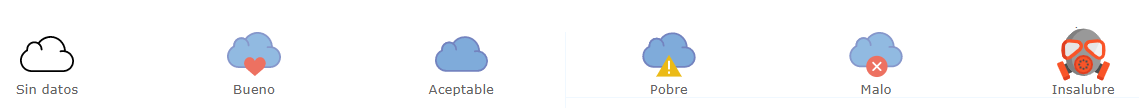
\includegraphics[width=10cm]{EAQI_Icons}
    \caption{Iconografica Aire Guru}
\end{figure}

Para las graficas que muestran variaciones en el tiempo, se han utilizado graficos de lineas, que son las mas apropiadas para este tipo de datos,
ya que muestran la continua evolucion durante un periodo de tiempo. Para representar los distintos componentes del AQI se ha utilizado un
grafico de barras apiladas, ya que se ve que proporcion del AQI total esta formada por que contaminante.\\
\begin{figure}[ht]
    \centering
    \subfigure[AQI Evolution]
     {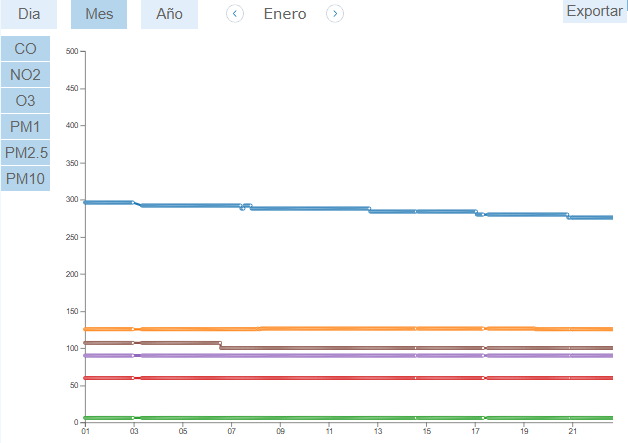
\includegraphics[width=5.75cm]{lineChart}}
     \hfill
     \subfigure [AQI components]
    { 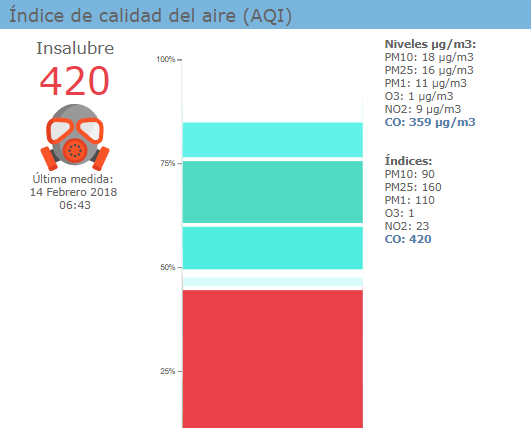
\includegraphics[width=5.25cm]{stakedBarChart}}
 
    \caption{Charts}
\end{figure}

Ademas, para explicar el concepto de AQI y crear un awarnes sobre la influencia que tiene en nosotros la polucion del aire, Aire Guru proporciona un 
glosario y una ayuda con las descripciones de los agentes contaminantes, complicaciones medicas, fuentes de contaminacion, la iconografia utilizada y
una explicacion sobre que es y como se calcula el AQI.\\

 
\elsparagraph{Evaluation}  
\begin{itemize}
    \done El lenguaje utilizado en toda la herramienta es un lenguaje comun, huye de la terminologia cientifica pero proporciona la informacion
    suficiente para enteder la situacion.
    \done Se han estudiado y utilizado las graficas mas apropiadas para cada tipo de datos.
    \crossed Algunos terminos especificos no se han podido sustituir como "Indice de calidad del Aire".
    \done Se han proporcionado la herramientas necesarias para entender el concepto. Se ha utilizado la norma europea de calidad del aire para 
    representar los valores y se ofrece al usuario recursos en la pagina para su comprension ademas de recursos extenos.
    
\end{itemize}
 

\newpage
\subsection{Interpretacion de los datos. Vocabulario y terminologia}

Recordemos que el objetivo principal del acceso a los datos, es obtener conocimiento. Hay que tener en 
cuenta que los datos por si solos, no tienen ningun valor, ya que carecen de sentido, una vez integrados en un contexto,
nos aportara informacion, y procesando y analizando esta informacion, se obtendra el conocimiento.\\
    
\begin{figure}[ht]
    \centering 
    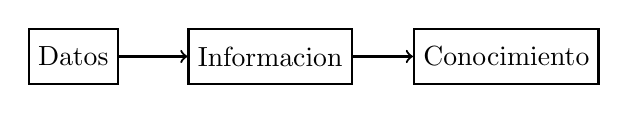
\begin{tikzpicture}[thick]
        \node[draw,rectangle,minimum size=20] (a) {Datos};
         \node[draw,rectangle,minimum size=20,right of= a, node distance=2.5cm] (b) {Informacion};
         \node[draw,rectangle,minimum size=20,right of=b, node distance=3cm] (c) {Conocimiento};
         \draw[->] (a) to (b);
        \draw[->] (b) to (c);
     
      \end{tikzpicture}
      \caption{Diagrama. De datos a conocimiento}
    \end{figure}
 
Para poder obtener este conocimiento de los datos, es necesario que el usuario interprete correctamente los datos, por lo
que el usuario debe contar con conocimientos en la materia o realizar una tarea de investigacion, que le permita 
entender los datos extraidos. 

Asi pues, para que el usuario pueda obtener la informacion de una manera directa, requiere de conocimientos tanto 
de programacion como especificos de la materia y los recursos para crear una infraestructura que le permita implementar 
una representacion de los datos que le sea util.

Podemos concluir que el acceso a los datos por parte del usuario medio, no es directa.\\

Para poder construir un sistema que haga los datos accesibles, es imprescindible disenar un modelo  para concretar la 
informacion que se desea obtener. El diseno de un sistema permitira que a partir de unos valores dados, proporcione unos resultados.
Para ello sera necesario tener un conocimiento solido del conjunto de datos que se necesita, los valores,
sus unidades y como se relacionan entre si.


\subsubsection{How to solve it} 
Estudiar el objetivo buscado y recurrar a la ayuda de expertos si fuera necesario para adquirir los conocimientos necesarios
sobre la materia. Disenar un modelo que proporcione la informacion que buscamos. Este modelo debera proporcional la informacion 
al usario en un lenguaje o formato compresible. Si no es posible proporcionarmos las herramientas necesarias para que este pueda 
comprender el contexto de la informacion.

\subsubsection{How we solve it. Aire Guru} 
Aire Guru se ocupa de representar el EAQI (European Air Quality Index) general calculado sobre un mapa. Este es un formato mas legible para los usuarios.
Este indice mustra un indicador con cinco niveles: "Insalubre" "Malo" "Pobre" "Aceptable" y "Bueno" y especifica un rango de colores desde el rojo hasta el celeste.\\
\newpage
\begin{figure}[ht]
    \centering
    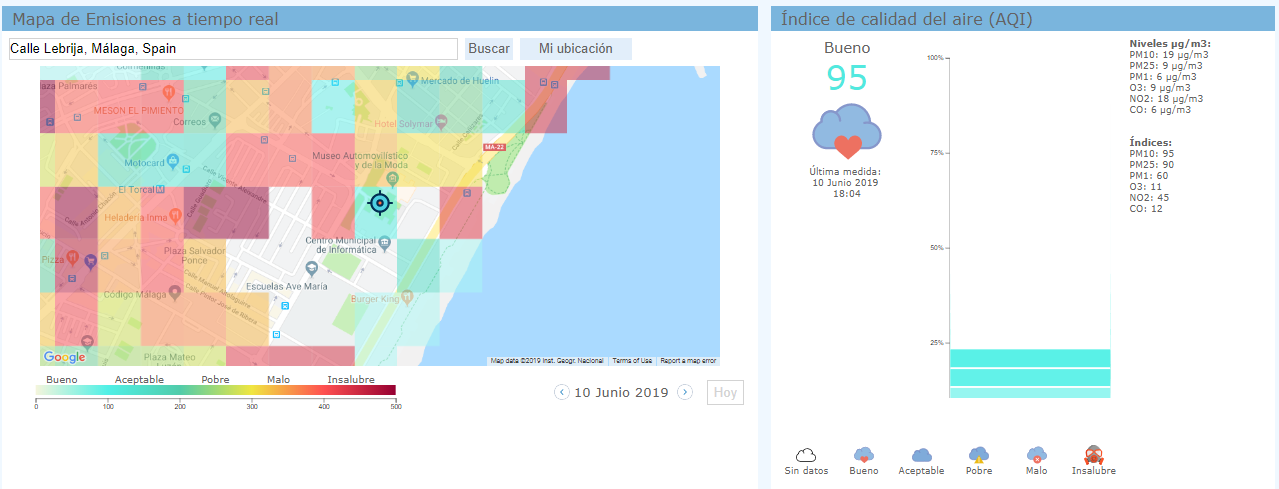
\includegraphics[width=10cm]{mapAireGuru}
    \caption{Aire Guru. Landing page. Top section}
\end{figure}

Nuestra plataforma introduce ademas una iconografica para ayudar al usuario a tener una idea directa de la situacion, ya que son mas 
explicativos que los colores. En caso de peligro, queda bien representado con el color rojo, pero en el caso del azul o verde, en nuestra cultura, no
tenemos definido un estado para estos colores.\\
\begin{figure}[ht]
    \centering
    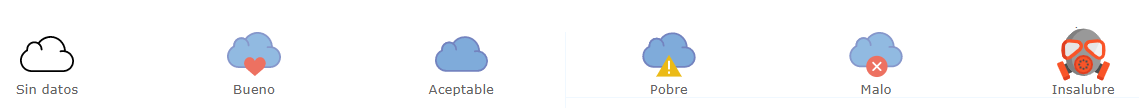
\includegraphics[width=12cm]{EAQUI_Icons}
    \caption{Iconografica Aire Guru}
\end{figure}

Ademas proporciona un glosario con las descripciones de los agentes contaminantes, complicaciones medicas, fuentes de contaminacion
y la iconografia utilizada y una ayuda donde se puede consultar el calculo de AQI y ampliar informacion.

La herramienta Aire guru presenta la informacion en el idioma nativo de la ciudad y se utiliza un lenguaje sencillo y directo.
Ademas se utiliza el mismo estilo, colores e iconografia en todo el diseno para que el usuario se familierize rapidamente y pueda
prestar atencion al significado de los datos en vez de perderse en el diseno e intentar encontrar su significado.

Aire Guru se comprende de distintas secciones disponibles para todos los usuarios. En la zona superior, podemos ver el mapa que mediante la seleccion de un punto, nos
mostrara informacion detallada de este punto. A continuacion, cuenta con una seccion que filtrara la informacion acorde a las preferencias del usuario
y para concluir, muestra el historial de los contaminantes desde 2018.
Ademas, para usuarios identificados, mostrara directamente la informacion de su localizacion y mostrara al usuario su historial personal
con la polucion a la que ha estado rodeado.

El workflow de las distintas secciones de Aire Guru esta detalladamente estudiada. Como vemos en la Figura X. Aire Guru. Landing page. Top section, el punto de partida es la localizacion que nos interesa,
a continuacion se muestra la informacion general de este punto, el AQI general, despues el AQI de cada uno de los contaminantes que componen el 
AQI general y por ultimo los valores numericos de cada uno de los contaminantes. Como vemos vamos de menos a mas detalle.

\paragraph{Evaluation} \mbox{} 

\begin{itemize}
\done El lenguaje utilizado en toda la herramienta es un lenguaje comun, huye de la terminologia cientifica pero proporciona la informacion
suficiente para enteder la situacion.
\crossed Algunos terminos especificos no se han podido sustituir como "Indice de calidad del Aire".
\done Se han proporcionado la herramientas necesarias para entender el concepto. Se ha utilizado la norma europea de calidad del aire para 
representar los valores y se ofrece al usuario recursos en la pagina para su comprension ademas de recursos extenos.
\end{itemize}

\newpage
\subsection{Optimizacion de la accesibilidad}

Para ofrecer los datos a los usuarios de una manera directa, es recomendable utilizr una plataforma a la que el usuario
este familiarizado. Por ejemplo, es mas factible que el usuario se sienta mas atraido a acceder a los datos si no requiere
ninguna instalacion en sus dispositivos.\\

-- Instalacion de dispositivos para extraer la informacion ellos mismos


\subsubsection{How to solve it} 
Ofrecer la informacion mediante una pagina web o una aplicacion movil. Ofrecer toda la informacion posible sin necesidad de
hacer que el usuario realize acciones complicadas, como la identificacion.
Ofrecer una plataforma segura.

\subsubsection{How we solve it. Aire Guru} 

Para garantizar el alcance a la mayoria de la poblacion, Aire Guru esta disponible en las direcciones webs https://www.aire.guru y https://www.airquality.guru.
Usa SSL que garantiza la encriptacion de los datos atraves de la red, ademas, cada vez mas navegadores intentan proteger a los usuarios y
solo muestran paginas que utilizar un metodo seguro. 

Como comentabamos anteriormente, todos los usuarios pueden ver la informacion basica sin necesidad de aportar ningun dato o identificarse, sin la necesidad de 
realizar ninguna descarga o instalacion y hoy en dia, casi todo el mundo esta familiarizado con la navegacion web.

\elsparagraph{Evaluation}  

Ofrecerles a los usuarios una pagina web libre de cargos, facilita que el usuario acceda directamente a la informacion
sin tener que realizar ninguna descarga. Al eliminar esta barrera, el usuario nos da un punto de confianza.
--reacio a identificarse
--y actualmente se esta trabajando en su traduccion al ingles, para cubrir un rango mas amplio de su poblacion, ya que esta ciudad es cada vez mas cosmopolita.
\\newpage





\begin{comment}
    

    ----Respecto a polucion del aire 
    Acudir a fuentes privadas
    Instalacion de dispositivos
  Done-  Ejemplos de bases de datos de distintas ciudades capitales


    --no plataformas de pago
Done -no instalacion de software
-no complicaciones por parte del usuario.

--Datos automatizados -- formato maquina
--almacenamiento
--conocimientos informaticos
--analiticos
--estudio de la materia, ver que es importante o no, contrastarlo
--equipo multidisciplinario
--informaticos no son expertos en medicina, por ejemplo.
\begin{itemize}

    \item datos disponible
    \item no substraible por el usuario medio
    \item imposible de tratar sin una estructura
    \item no es posible de tener un historico
    \item sin informacion complementaria que muestre informacion util
    \item Desperdicio
    \item \end{itemize}

---Si fuera necesario, se le puede proporcionar las herramientas para que pueda entenderlo, en los 
casos mas complicados donde se necesitan conocimientos previos sobre la materia.

---Incluir concepto de muestras
\end{comment}  
    
